\section{Getting Started}
\label{sec:getting_started}

\subsection{What is mbed?}
\label{sub:what_is_mbed}
\begin{frame}
	\frametitle{What is mbed?}
	The mbed platform is a collection of open source hardware and software to allow rapid ARM based prototyping
	\begin{itemize}
		\item Professional online compiler lets you work from any computer
		\item Integrated version control system lets you easily find and use libraries
		\item CMSIS based APIs let you work high level or bare metal
		\item Hardware abstraction layer insulates your application from hardware changes
	\end{itemize}
	\textit{Essentially a high performance Arduino with highly integrated tools to save you time!}
\end{frame}

\subsection{mbed.org}
\label{sub:mbed_org}
\begin{frame}
	\frametitle{Register on mbed}
	\begin{columns}[c]
		\begin{column}{0.5\textwidth}
			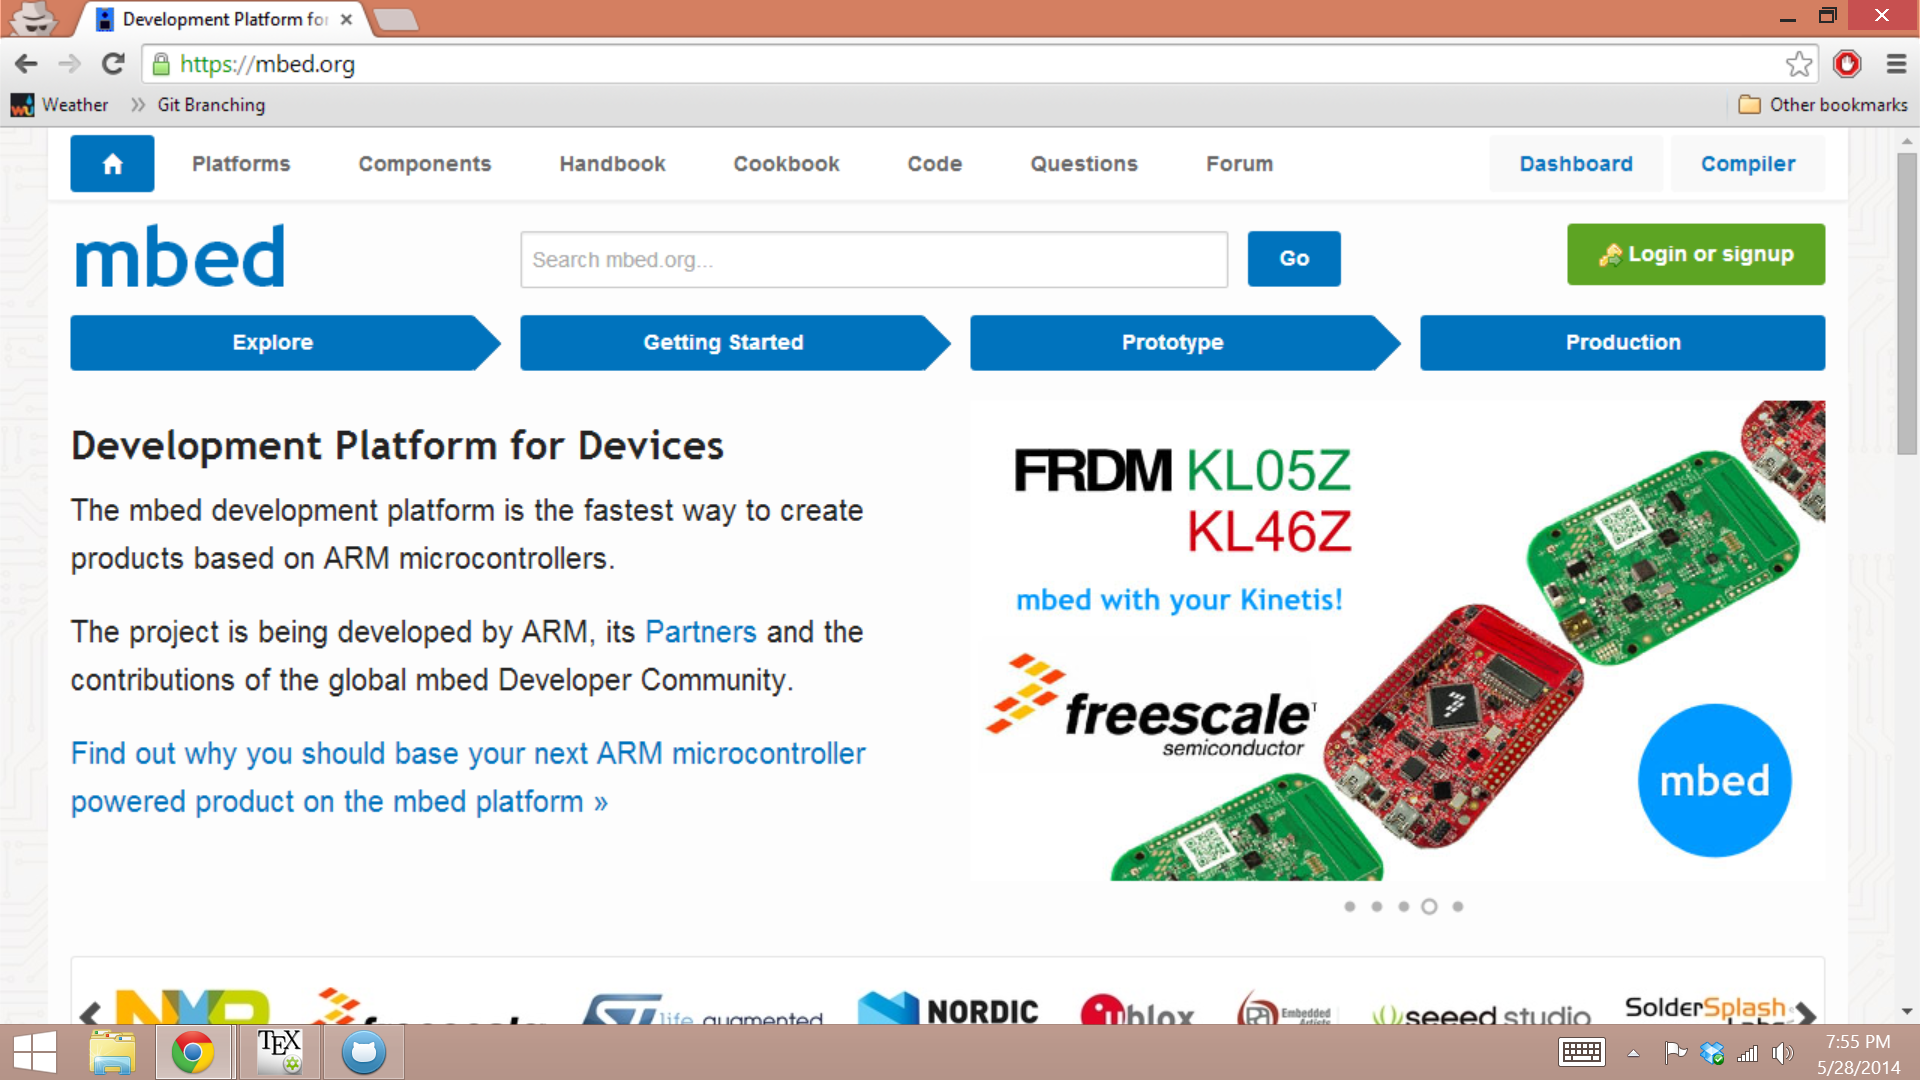
\includegraphics[width=\linewidth]{mbed_register}
		\end{column}
		\begin{column}{0.5\textwidth}
			\begin{enumerate}
				\item Navigate to \url{http://www.mbed.org}
				\item Click the green "Login or signup" button
				\item Click the "Signup" button
				\item Follow the prompts
				\item Confirm your e-mail address
			\end{enumerate}
		\end{column}
	\end{columns}
	\begin{center}
		Everyone should have an mbed account.
		You can create a team to share code between members of your organization.
	\end{center}
\end{frame}

\subsection{Nucleo Development Board}
\label{sub:nucleo}
\begin{frame}
	\frametitle{Nucleo Development Board}
	\begin{columns}[T]
		\begin{column}{0.5\textwidth}
			The Nucleo development board combines a USB programmer with a powerful STM32 processor and Arduino compatible headers
			\begin{itemize}
				\item ARM Cortex-M4 with FPU at 84 MHz
				\item 512 KBytes of flash memory
				\item 12 bit ADC at 2.4 Msps with up to 10 channels
				\item Up 3xUART, 3xI2C, 4xSPI interfaces
			\end{itemize}
		\end{column}
		\begin{column}{0.5\textwidth}
			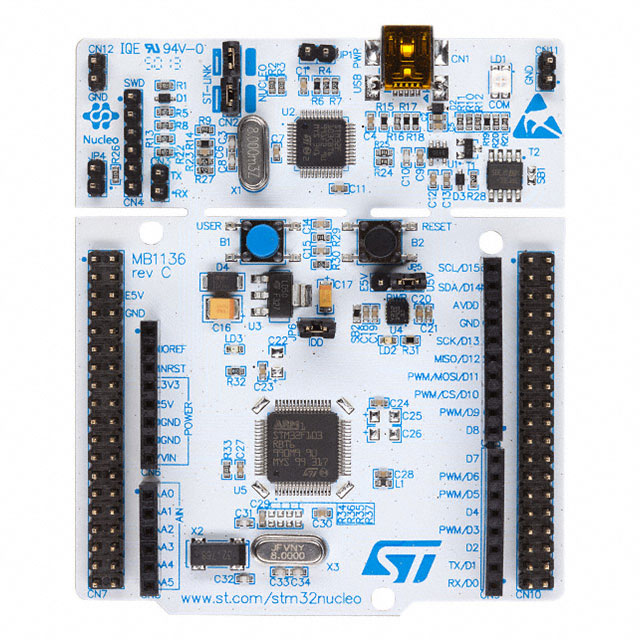
\includegraphics[width=\linewidth]{nucleo}
		\end{column}
	\end{columns}
\end{frame}

\begin{frame}
	\frametitle{Add Nucleo to Your Account}
	\begin{columns}[c]
		\begin{column}{0.5\textwidth}
			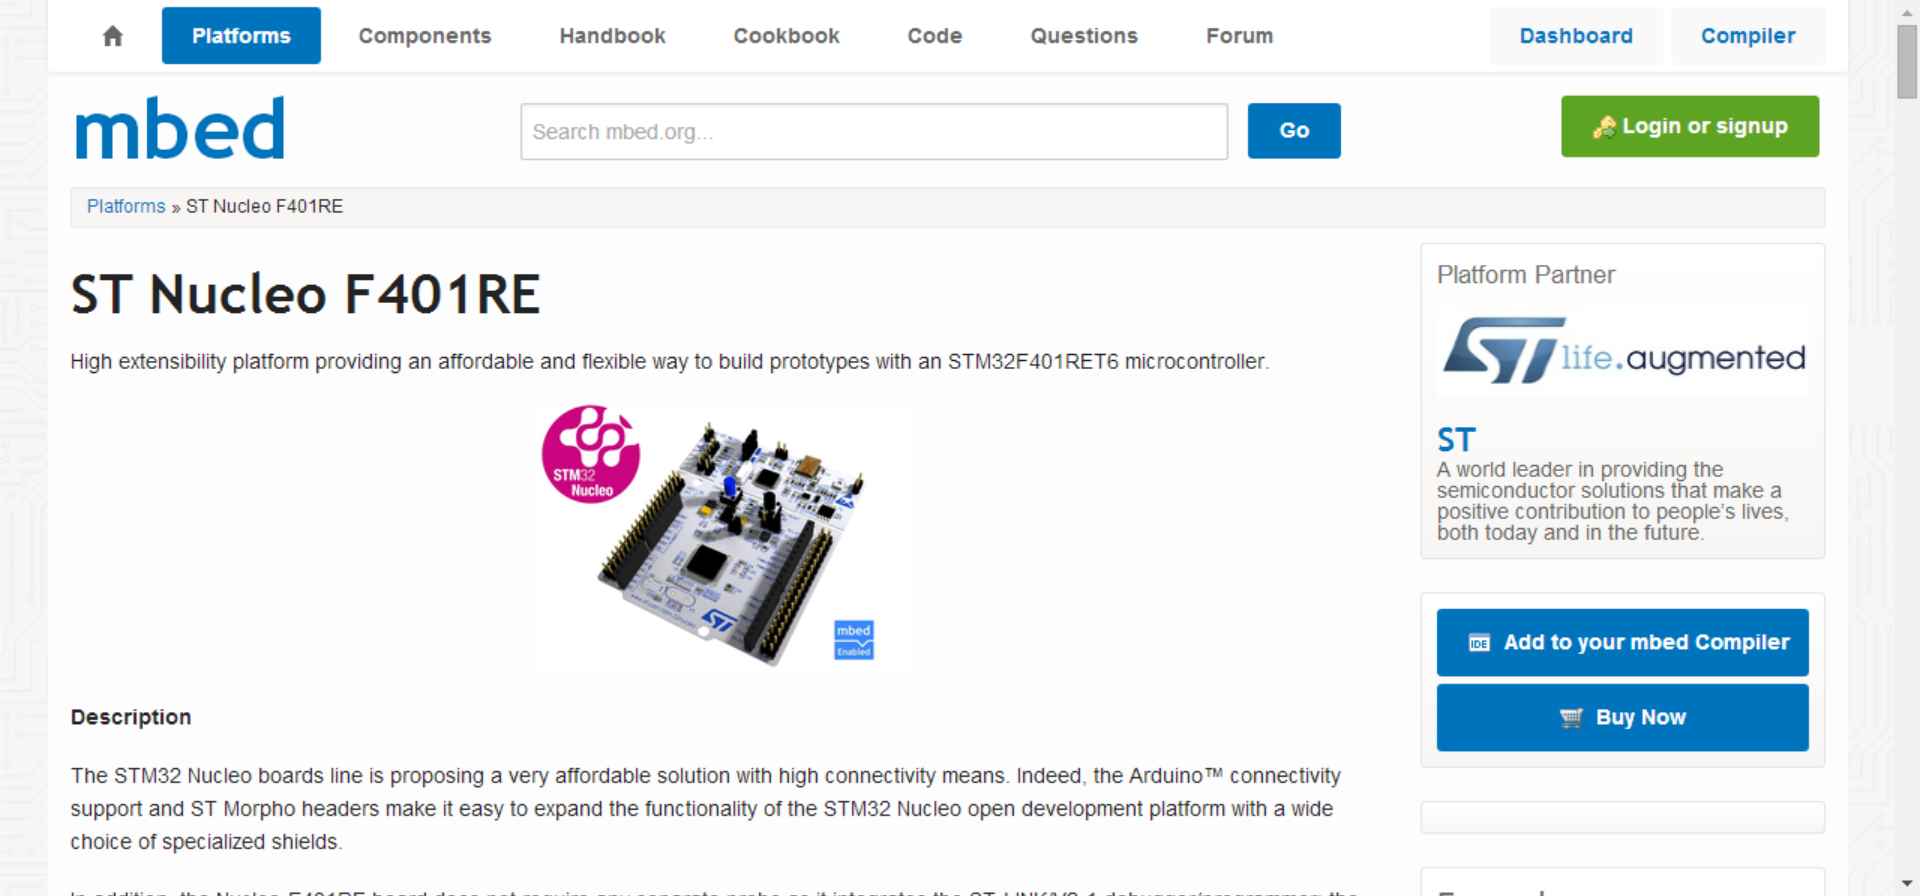
\includegraphics[width=\linewidth]{add_nucleo}
		\end{column}
		\begin{column}{0.5\textwidth}
			\begin{enumerate}
				\item Connect your Nucleo to your computer
				\item Open the external drive the connects
				\item Double click the mbed.htm file
				\item Click "Add to your mbed Compiler"
			\end{enumerate}
		\end{column}
	\end{columns}
	\begin{block}{Note}
		You only need to do this once per account!
	\end{block}
\end{frame}

\begin{frame}
	\frametitle{Install Drivers}
	Drivers are needed to access the Serial port on the Nucleo.  You can find drivers at this URL: \url{http://www.st.com/web/en/catalog/tools/PF260218}.  These drivers are for Windows Vista, 7 and 8. \ \\ \ \\
	\begin{block}{Note}
		Programming the Nucleo does not require drivers since the board shows up as a Mass Storage Device.
	\end{block}  
\end{frame}

\begin{frame}
	\frametitle{Additional Resources}
	Additional resources such as datasheets, product sheets, schematics and firmware can be found at the URL below.
	\url{http://www.st.com/web/catalog/tools/FM116/SC959/SS1532/LN1847/PF260000}
	\begin{block}{Note}
		Programming the Nucleo does not require drivers since the board shows up as a Mass Storage Device.
	\end{block}  
\end{frame}